\chapter{Landasan Teori}
\label{chap:pendahuluan}

\section{Mesin Navigasi KIRI}
\label{sec:mesin_navigasi_kiri}

KIRI memiliki mesin navigasi yang dibangun pada bahasa Java. Mesin ini bertugas
untuk menerima masukan berupa koordinat titik asal dan tujuan, kemudian
menemukan angkot-angkot yang harus dinaiki untuk menuju titik tujuan dari
titik asal. Karena alasan kerahasiaan, pembahasan mengenai mesin navigasi
KIRI tidak mengacu pada referensi publik, melainkan dari survei terhadap
kode sumber internal KIRI.

\begin{figure}
\centering
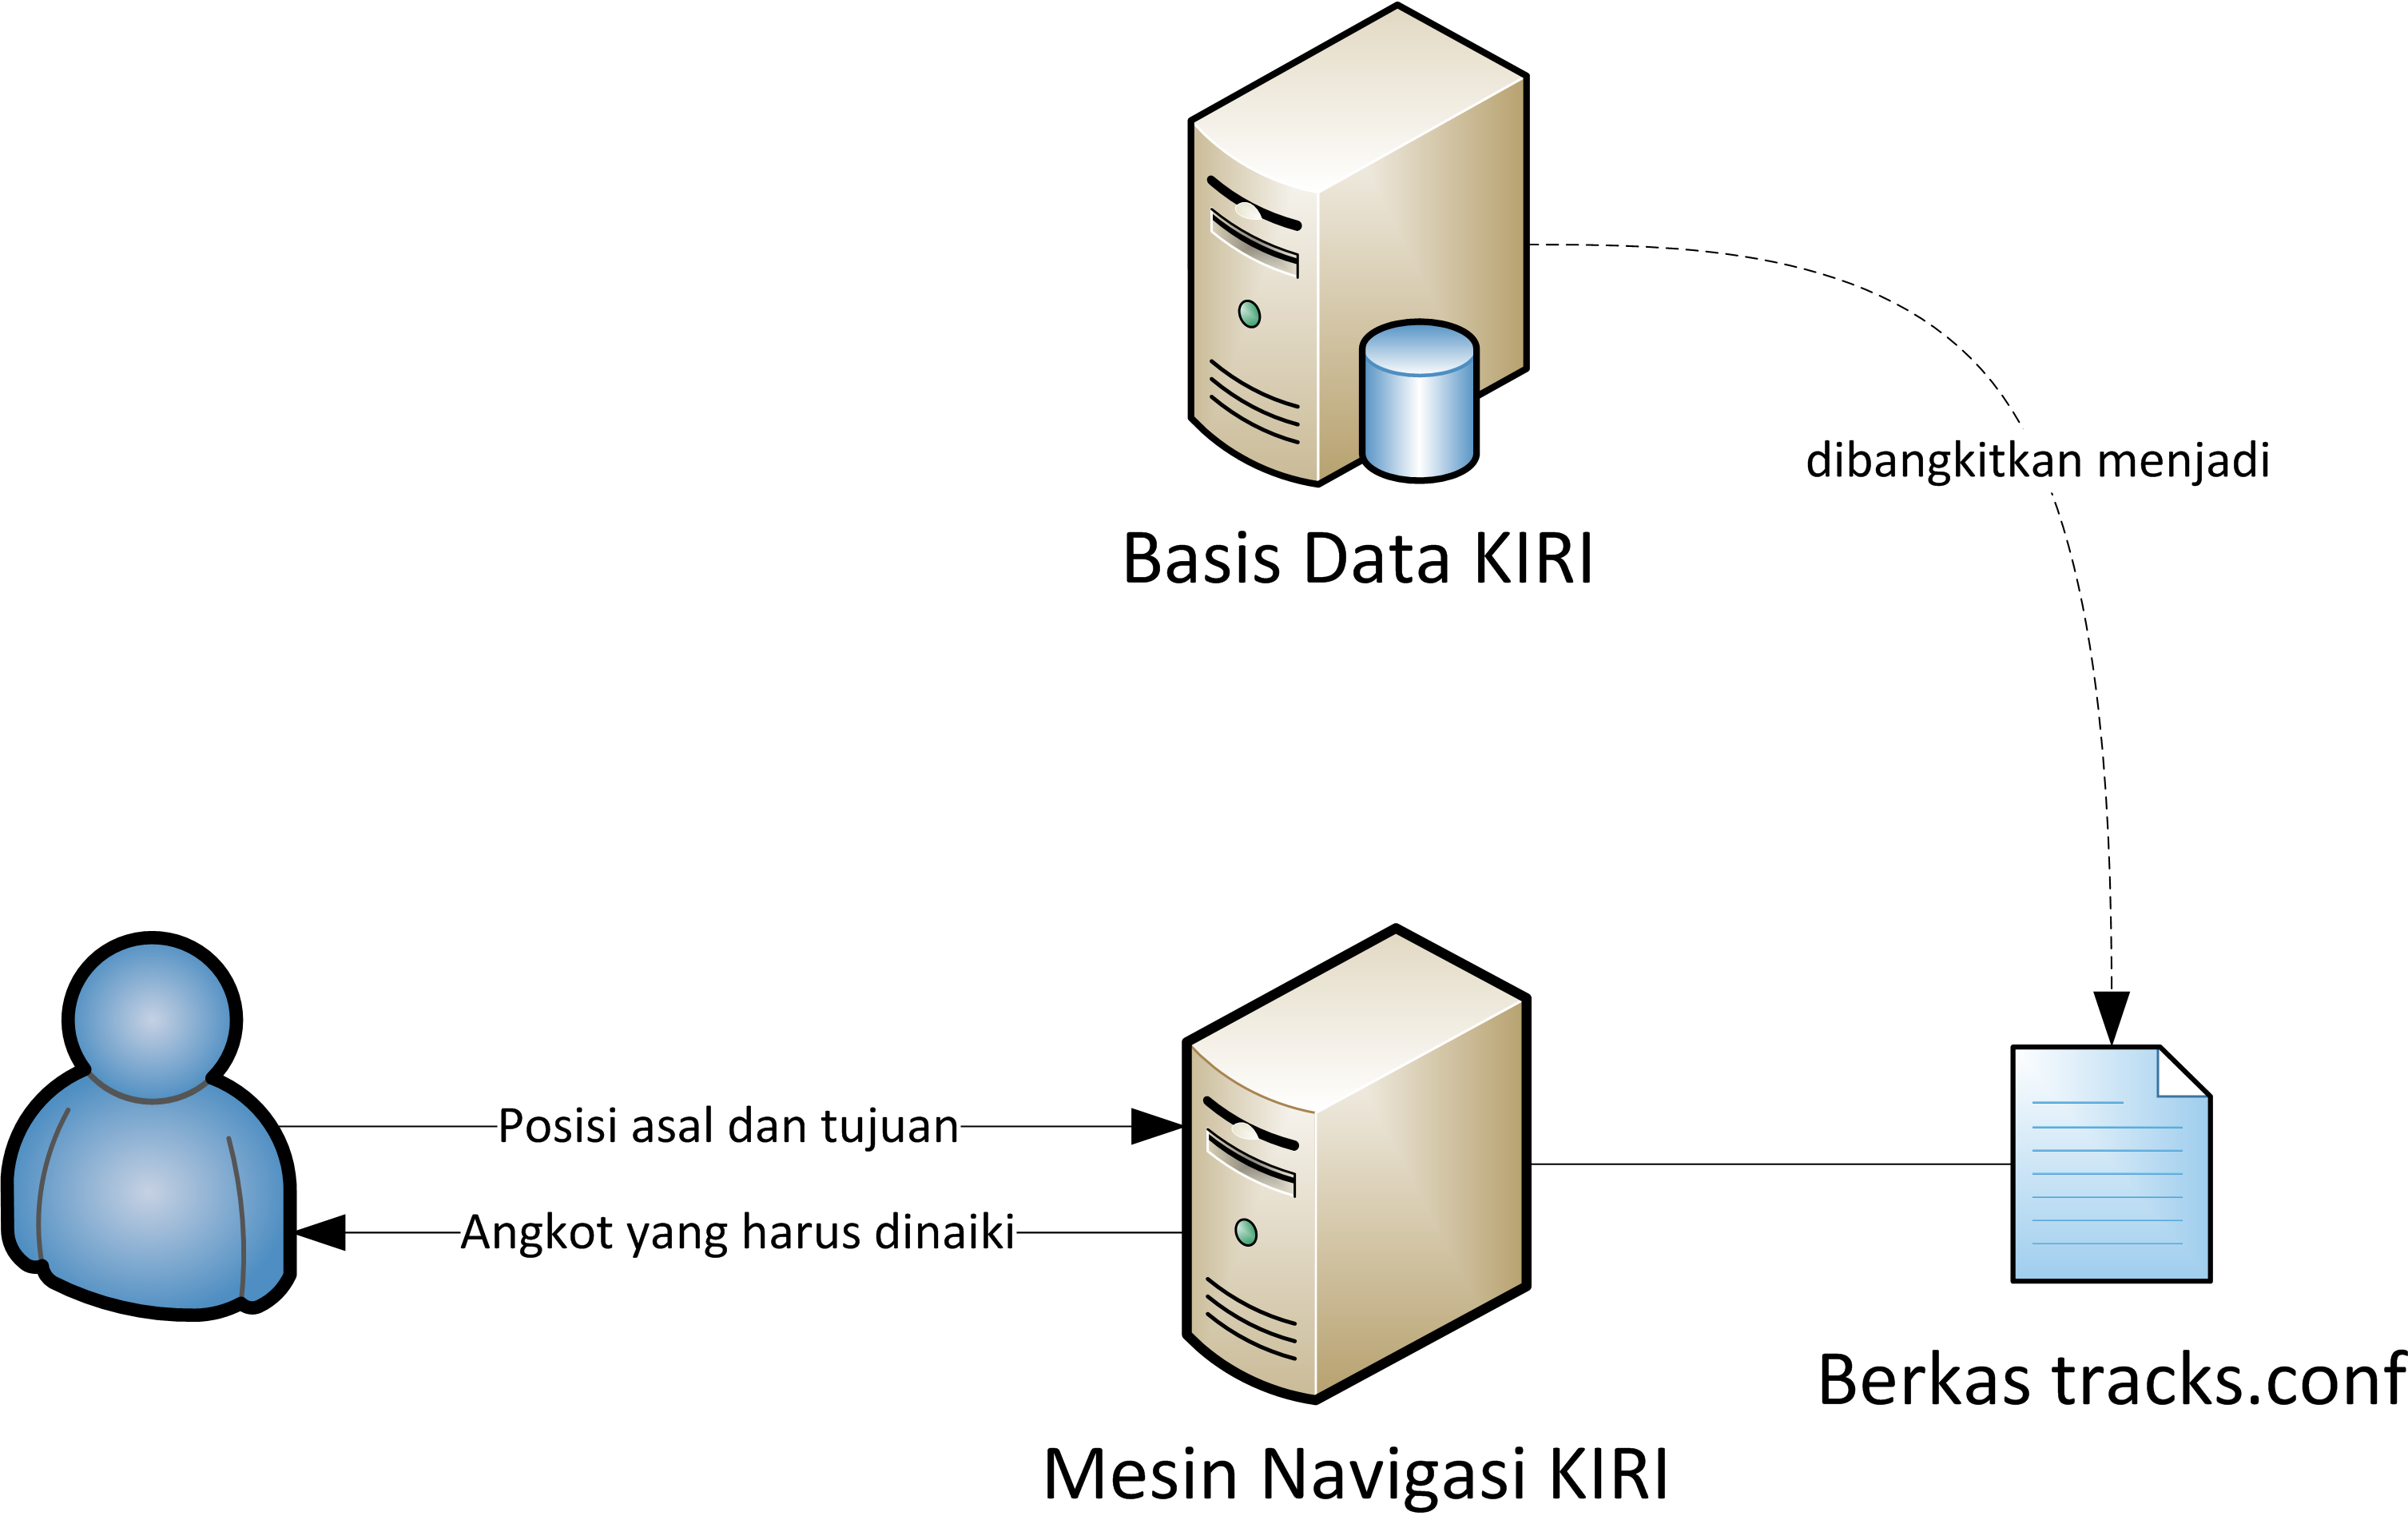
\includegraphics[scale=1]{Gambar/2_arsitektur_saat_ini}
\caption{Arsitektur Saat Ini} 
\end{figure}

Seperti dapat dilihat pada gambar \ref{fig:2_arsitektur_saat_ini}, elemen
arsitektur yang mendukung navigasi KIRI dibagi menjadi tiga, yaitu:
\begin{itemize}
	\item \textbf{Basis Data KIRI} menyimpan informasi rute 33 trayek angkot,
		yang masing-masing mencakup identifikasi trayek (\verb/trackId/ dan
		\verb/trackTypeId/), nama trayek (\verb/trackName/), daftar koordinat
		yang dilewati (\verb/geodata/), informasi pulang-pergi
		(\verb/pathloop/), catatan internal (\verb/internalInfo/), prioritas
		untuk dipilih (\verb/penalty/), informasi naik/turun penumpang
		(\verb/transferNodes/), dan parameter ekstra untuk pembelian
		tiket (\verb/extraParameters/).
	\item \textbf{Berkas tracks.conf} adalah hasil ekstraksi dari basis data
		kiri, yang menyimpan informasi penting saja yang dibutuhkan oleh algoritma
		mesin navigasi KIRI, yakni: \verb/trackId/, \verb/trackTypeId/,
		\verb/penalty/, \verb/geodata/, \verb/pathloop/, dan
		\verb/transferNodes/.
	\item \textbf{Mesin Navigasi KIRI} adalah program yang bertugas mengolah
		data yang ada pada berkas tracks.conf, sehingga dapat menjawab
		pertanyaan navigasi dari titik asal ke titik tujuan. Karena alasan
		historis, mesin navigasi tidak membaca data langsung dari basis data,
		melainkan dari berkas tracks.conf.
\end{itemize}

\subsection{Basis Data KIRI}
Basis data KIRI disimpan dalam sistem basis data MySQL. Salah satu dari
tabel yang digunakan adalah tabel \verb/tracks/, yang menyimpan informasi
rute trayek. Struktur dari tabel ini dijelaskan pada tabel
\ref{tab:2_struktur_table_tracks} berikut.

\begin{table}
	\begin{tabular}{|p{2.5cm}|p{2.5cm}|p{10cm}|}
		\hline
		Nama kolom & Tipe & Keterangan \\
		\hline
		trackId & varchar(32) & Kode trayek angkot (misal: "sthallciumbuleuitlurus").
			Menjadi PRIMARY KEY tabel bersama trackTypeId. \\
		trackTypeId & varchar(32) & Kode tipe trayek (untuk angkot bandung,
			selalu berisi "bdo\_angkot"). Menjadi PRIMARY KEY bersama trackId. \\
		trackName & varchar(32) & Nama trayek yang dapat dibaca secara umum
			(misal: "St. Hall - Ciumbuleuit (lurus)"). \\
		internalInfo & varchar(1024) & Informasi internal yang dapat
			ditambahkan dan tidak akan ditampilkan pada hasil pencarian. \\
		geodata & linestring & Daftar koordinat dari rute trayek ini. \\
		pathloop & tinyint(1) & Menandakan apakah trayek ini adalah trayek
			pulang pergi atau satu arah. \\
		penalty & decimal(4,2) & Bobot dari trayek ini. Semakin besar nilainya,
			semakin kecil kemungkinan akan muncul pada hasil navigasi. \\
		transferNodes & varchar(1024) & Daftar indeks titik di mana penumpang
			dapat turun maupun naik, dipisahkan dengan koma. Untuk angkot
			Bandung, penumpang dapat turun dan naik di semua titik. \\
		extraParameters & varchar(256) & Informasi yang ditambahkan saat
		melakukan pembelian tiket (tidak terkait dengan penelitian ini). \\
		\hline
	\end{tabular}
	\caption{Struktur Tabel tracks}
	\label{tab:2_struktur_tabel_tracks}
\end{table}

\subsection{Berkas tracks.conf}

\subsection{Mesin Navigasi KIRI}

\section{Protokol angkot.web.id}
\label{sec:mesin_navigasi_kiri}
